\documentclass{article}
\usepackage[margin=1in]{geometry}
\usepackage{graphicx}
\usepackage{hyperref}
\usepackage{float}
% \usepackage{setspace}
% \onehalfspacing
% \allowdisplaybreaks
%

\begin{document}
\begin{titlepage}
  \centering
  \hphantom{}\par
  \vspace{2cm}
  
\includegraphics[width=0.15\textwidth]{logo.png}\par\vspace{0.5cm}
  {\LARGE \textsc{University of Oxford}\par}\vspace{0.5cm}
  {\Large \textsc{Group Design Practical}\par}\vspace{0.5cm}
  {\large \textsc{Group 14}\par}\vspace{0.7cm}
  {\Huge Machine Learning in the Browser with the BBC Micro:Bit\par}\vspace{0.8cm}
  {\large Louis-Emile Ploix\footnote{\href{mailto:louis-emile.ploix@stcatz.ox.ac.uk}{louis-emile.ploix@stcatz.ox.ac.uk}}, Ike Glassbrook\footnote{\href{mailto:isaac.glassbrook@lmh.ox.ac.uk}{isaac.glassbrook@lmh.ox.ac.uk}}, Joseph Simkin\footnote{\href{mailto:joseph.simkin@some.ox.ac.uk}{joseph.simkin@some.ox.ac.uk}}, Alikhan Murat\footnote{\href{mailto:alikhan.murat@magd.ox.ac.uk}{alikhan.murat@magd.ox.ac.uk}}, Andy van Horssen\footnote{\href{mailto:andy.vanhorssen@sjc.ox.ac.uk}{andy.vanhorssen@sjc.ox.ac.uk}}, and Ewan Hawkrigg\footnote{\href{mailto:ewan.hawkrigg@keble.ox.ac.uk}{ewan.hawkrigg@keble.ox.ac.uk}}\par}\vspace{0.7cm}
  {\large Internal supervisor: Qian Xie\par \vspace{0.3cm} External supervisor: Robert Knight \par}\vspace{1cm}
  {\Large May 2024}
\end{titlepage}

\tableofcontents

\section{Introduction}%
\label{sec:intro}

The Group Design Practical is a course taken by all 2nd year undergraduate students at the University of Oxford studying for a degree in Computer Science, Mathematics and Computer Science, or Computer Science and Philosophy. This report details the work of Group 14 from February to May 2024 to design, implement, and deploy a product satisfying the specification as provided by Micro:Bit. \\

The project itself may be viewed on the page \url{https://ox24-cctd-ml-machine.pages.dev}, and the source code is publicly accessible at \url{https://github.com/Ike-G/ox24-cctd-ml-machine}.

\subsection{Technical context}%
\label{subsec:context}

Our project is based on a machine learning tool developed by researchers at the Centre for Computational Thinking and Design at Aarhus University. This tool is publicly deployed at \url{https://ml-machine.org}, with its source code available at \url{https://github.com/microbit-foundation/cctd-ml-machine}. Our project is a fork of this repository, extending the existing project. \\

ML-Machine is an application for users with access to a physical micro:bit device to train a machine learning model that uses the micro:bit's sensors as input data. The user is given a 3 step process:
\begin{enumerate}
        \item Named `Gestures' are added, for the trained model to eventually use as classification categories. The user then adds to each gesture several recordings of the accelerometer that correspond to the particular gesture. Alternatively, they can use the example dataset, containing the categories `shake' (with recordings of the micro:bit being shook), `still' (with recordings of the micro:bit not moving), and `circle' (with recordings of the micro:bit being moved in a circle).
  \item The user trains a model -- either a dense layers model, or a k-nearest neighbours model -- to classify the data. The recordings are pre-processed using a set of filters, which build the feature set. Before training, the user may select in particular which filters they would like to use.
        \item The micro:bit then has its sensors periodically polled in order to predict, of the labelled gestures, the one most similar to its current movement.
\end{enumerate}

The web application is written using the Svelte framework~\cite{svelte}, acting essentially as an HTML template language. The micro:bit itself requires additional drivers to interface with the application, as first a bluetooth connection must be established, and then the appropriate sensor data must be streamed to the application. These are written in C++, and then converted into \verb|.hex| files, which users can install on their micro:bits in order to allow this procedure to work. Both models are trained in the browser using TensorFlow.js~\cite{tensorflowjs}. \\

% Detail the current state, explaining the work of Aarhus University
% Explain the initial build of the project

\subsection{Project Specification}%
\label{subsec:spec}

In consideration of the existing context, the specifications set out by Micro:Bit were designed with a view to utilise our work for experimental purposes, and to provide a benchmark for evaluating the feasibility of future projects. On this basis, the specification gave the following requirements of a final product:
\begin{itemize}
  \item That a user should be able to train any model on not just the micro:bit's accelerometer, but also an additional sensor.
        \begin{itemize}
                \item The user should be able to choose which sensor's data is to be streamed into the training data (and thus, which sensor's data is polled once the model is trained).
                \item Information given by the sensor should be visualised to the user in real-time in a manner which is understandable.
                \item The sensor data should be amenable to machine-learning analysis via the models available.
        \end{itemize}
  \item In addition to the Dense Neural Network, and the k-Nearest Neighbours models of the base application, a new neural network architecture should be investigated for implementation.
        \begin{itemize}
                \item This network should be capable of predicting on simple patterns with reasonable accuracy.
                \item The technical details of the network should be of pedagogical value, in addition to being amenable to high-level explanation.
                \item The trained model should be of a size that could fit on the micro:bit itself, rather than needing to run on a connected device\footnote{The Micro:Bit team have expressed a desire to run the prediction models directly on the micro:bit in future, rather than in the browser, allowing for the model to be stored independently of the application. This was not itself within the scope of our specification however.}.
                \item Model training should be responsive on standard browsers ran on computers with low-end modern hardware.
        \end{itemize}
\end{itemize}

\section{Logistics}%
\label{sec:logistics}

This section describes the timeline of our development, and how we went about structuring the delegation of work.

\subsection{Timeline}%
\label{subsec:timeline}

\begin{itemize}
        \item 24th January -- First briefing meeting, team members were introduced to one another, and communication channels were created.
        \item 26th January -- First internal meeting, we decided on our three preferred projects, one of which was the project we were ultimately assigned.
        \item 20th February -- First meeting with both supervisors. The project and existing code were explained, with directions given to relevant tools. It was decided that two weeks were to be given to all group members to analyse and understand the existing code, and decide on their areas of focus.
        \item 3rd March -- Project repository fork was created at \url{https://github.com/Ike-G/ox24-cctd-ml-machine}.
        \item 5th March -- Initial internal meeting to organise plans for initial development over the Hilary vacation. Plans were set to have weekly internal meetings, and weekly external meetings, on Mondays and Tuesdays respectively. An initial role distribution was decided.
        \item 9th March -- Beginning of Hilary vacation.
        \item 12th March -- Updated drivers to expose the magnetometer service. Consideration of initial ideas for new ML models.
        \item 18th March -- Introduced functionality to work with multiple sensor types, including addition of sensor visualisations.
        \item 24th March -- Improvements to magnetometer preprocessing.
        \item 25th March -- Implementation of ML training with multiple sensors.
        \item 31st March -- Implementation of filter UI with multiple sensors.
        \item 3rd April -- Deployed project as web application via Cloudflare.
        \item 7th April -- Added fully functional Mixture of Experts model.
        \item 9th April -- Work on implementing audio as a new sensor put to the side, focus placed instead on researching future solutions.
        \item 13th April -- Implemented sensor selection in the UI.
        \item 15th April -- Start of 0th week: added the light sensor, using previous work to implement sensor selection, visualisation, filtering, training, and predictions.
        \item 16th April -- Gave initial demonstration to developers at Aarhus University.
        \item 28th April -- Finalising quality of life changes. Focus placed on the final report.
\end{itemize}

\subsection{Role Delegation}%
\label{subsec:delegation}

Roles were initially distinguished to place focus separately on:
\begin{itemize}
  \item Implementing drivers.
        \begin{itemize}
          \item Louis -- Magnetometer (done directly through the Magnetometer service).
          \item Alikhan -- Microphone (done through \verb|UART|).
        \end{itemize}
  \item Joseph -- Implementing a new ML model.
  \item Ike -- Adding visualisation graphs of new sensors.
  \item Andy / Ewan -- Testing of existing code / improvements to sensor pre-processing.
\end{itemize}

As the project progressed, it was quickly identified that significant alterations to existing code were necessary to implement multiple sensors. Ike dealt with this primarily once basic visualisation had been dealt with. Additionally, Louis was able to implement the magnetometer driver very on in the process, and consequently quickly moved to working on pre-processing and testing. Later down the line the multisensor implementation required more extensive UI, which Ike and Louis dealt with together. \\

Due to the size of the job, after deciding with the rest of the team on a Mixture of Experts model as the best option, Joseph spent most of the project working on developing and upgrading the model. As part of this, he worked in conjunction with those developing new sensors as the processing methods were changed, and new sensors were implemented. \\

Ultimately, the group eventually decided not to pursue training on the microphone sensor, due to audio data presenting far more complex problems than had previously been dealt with in the other sensors. Alikhan thus refocused his work from that point on researching means of circumventing our problems for a future implementation by the original project's developers. Instead of audio data, Louis implemented a light sensor later on in the project, meaning the project concluded with three available sensor types.

\section{Implementation}%
\label{sec:implementation}

\subsection{Streaming of new sensors from the micro:bit}%
\label{subsec:streaming}
We added support for two new sensors to the application: The magnetometer and the light sensor. In each case the sensor data needed to be sampled on the micro:bit and sent over bluetooth to the browser which is using the Web Bluetooth API~\cite{bluetoothapi}. The magnetometer was straightforward in that it has a dedicated Bluetooth Service~\cite{microbitservices}, an API for which is provided by the Lancaster Universitiy micro:bit Runtime~\cite{magnetometerservice}. Light sensing has no associated bluetooth service, so we sent the sampled data manually instead: To do this we start a `fiber' (a lightweight thread) when the micro:bit boots. This fiber repeatedly samples the environment brightness, sends this to the UART and sleeps for a few milliseconds. \\

For both sensors, the incoming data in the browser will be parsed, normalised and finally sent to an associated LiveData buffer. The LiveData buffers act as the sources of data for several other components of the application. \\

Although ultimately unused, work was also done to allow for the streaming of microphone data from the micro:bit. Already present in the application is the UART service, being used to play audio when the micro:bit classifies a certain gesture, as determined by the user. In the reverse direction, this can be used to record audio entirely on the micro:bit hardware, then send an array of bytes (representing amplitudes) back to the application. In particular, inspiration was taken from the MakeCode source code~\cite{makecode} to use a StreamRecording class to asynchronously build the byte array.

\subsection{Normalisation of data}%
\label{subsec:datanorm}
The data received by the browser will be the raw data as read by the micro:bit. This means it needs to be processed before it can be fed into other regions of the application which expect values to be of a specific range. In particular the magnetometer presented difficulties in its sensitivity and discontinuity at times. \\

Our initial attempt was a straightforward division into the required range. This was extremely sensitive, but also jumped discontinuously at times. We subsequently tried a logarithmic scaling, but this suffered from largely the same problems. We then realised that dropping the sign of each component of the vector dealt with the discontinuous jumps. This suggested that we were treating the data as signed when it should have been unsigned, but this does not match with any of the internals or documentation of the micro:bit runtime. This too remained incredibly sensitive to even small movements. Finally, we settled on taking the \verb|atan2| of the absolute of each pair of components. This is nice in that it has a physical interpretation: the x component would be the compass heading, and the \verb|y|, \verb|z| components would be equivalents on other axis.

\subsection{Sensor choice in the UI}%
\label{subsec:sensorchoice}
After discussion with the micro:bit team, it was decided that we wanted to allow the user of the application to be able to select which combination of sensors they wanted to be able to train the model with. It was important that this was done without compromising UX: in particular we did not want to force the user to make a decision they did not necessarily understand at the time. This was accomplished by adding a new page to the start of the pipeline the user follows, in which the user was given a clear choice of options with sensible defaults and help options if they wanted them. If no sensors were selected the user would be unable to train or record any gestures, and would instead be invited to do so. We also added indicators to each stage of the pipeline to help the user understand which stages were using which sensors. This is something we found to be a problem when testing the application ourselves. Finally we decided that if the sensor selection was changed we would clear the currently trained model to ensure that confusion over what was being used was completely avoided. \\

\subsection{Multisensor processing}%
\label{subsec:multisensor}

One of the key modifications to the existing codebase made in this project was the allowance for multiple sensors. The base project functions entirely on the basis of accelerometer input, and thus the architecture is designed with the assumption that only a single sensor will ever be used. \\

At any point in time, the application holds a classifier, encapsulating a model which may either be trained or untrained. In particular, we want that this model should be trained on the currently selected sensors, and that once this is done the prediction polling is done feeding in the correct sensor data. We note that it's still possible for users to train a model, then go back and change the sensors. In such cases we need to identify the model as untrained, so as to avoid creating a discrepancy in the UI. \\

In order to do this, we hold the sensor choice as an aspect of the base model data. Any calls to train the model must be passed using the Classifier repository's \verb|trainModel| method, and within this we receive the stored sensor choices. Note that in the UI we disallow the user from continuing if no sensor has been selected, and thus while a person could theoretically use dev tools to bypass the restriction, in every other case we guarantee that the sensor choice given is a valid one. From here, training is relatively straightforward -- although the different sensors naturally have different characteristics, the existing array of filters serves to capture the range of behaviours, and thus we have left it unchanged. Consequently the only modification is in data shape, and this is something that our model training code already deals with automatically.

% includes filter adaptation

\subsection{Visualisation of new sensors}%
\label{subsec:sensorvis}

Excluding development tools, there are three locations in the application where sensor inputs are visualised:
\begin{itemize}
  \item in the data tab, as a list of graphs each containing a data sample for the row's gesture;
  \item in the bottom bar, giving the live stream of sensor inputs;
  \item in the filters tab, indicating how current sensor inputs are filtered through to the ML model.
\end{itemize}

While using the same underlying library for both (smoothie~\cite{smoothies}), the visualisation needs for the former two applications end up being quite different. In the former case, the graphs are far smaller, and so there's much less space to work with before the visualisation becomes cluttered. Additionally, the information conveyed in this graph needs to reflect the data in the gesture which will ultimately be used in applications. Consequently, we modify these graphs to remove unused sensors entirely, and have different sensors represented by strongly contrasting colours. \\

In the latter case, the application displays a graph of the data being received in the browser from the micro:bit. This initially just contained the \verb|x|, \verb|y|, \verb|z| components of the accelerometer. We found that after adding the magnetometer and light sensor to the graph it became quite difficult to read, with now 7 lines displayed on the same graph. To deal with this we split the graph into three smaller graphs, one for each sensor, stacked on top of one another. This is much clearer to the user. We also now gray out the graphs not currently selected. Note that this does not mean that the live data isn't being rendered anyway. This distinction is important to help indicate to the user that the application is recording data for gestures from each sensor regardless of whether it is currently being used. This means that the user can change the sensor selection without re-recording data. \\

Minimal addition work was required for modifying the filters tab, as we have an entire page dedicated entirely to the visualisation, and thus plenty of space to work with. Each filter produces a value along each axis, and thus for each included sensor we have an additional axis on which to represented the value produced by the filter. Thankfully, there was already some space available on the page, and thus we've extended this in exactly the expected way.

\subsection{Application deployment}%
\label{subsec:deployment}

So as to help us streamline the development process, and ensure that errors were picked up on early, we deployed the application using Cloudflare~\cite{cloudflare}. In order to build the application, we use \verb|svelte-check| to act as a linter and highlight any initial concerns. Following this, we run our tests, and then finally build the application. This was deployed via the github repository, and consequently each commit was automatically tested and marked on github with the result. \\

By having the project actively deployed, we were both able to easily give the micro:bit developers access to our work concurrently, as well as to immediately identify holes in our changes.

\section{Areas of Further Development}%
\label{sec:development}

While all tasks as given in the initial specification were ultimately fulfilled, there remain a couple main areas in which the project could continue to develop along the lines that we were given. The most significant of these is in relation to audio processing, which was a project ultimately deemed out of scope relatively late on in development, and therefore we consider a hypothetical implementation below. Also of consideration for future development, leading on from considerations relating to audio, is the potential for modifications to filters in order to improve performance, which were largely left untouched during the development process.

\subsection{Audio processing}%
\label{subsec:audio}

Continuing from the implementation of audio as described in~\ref{subsec:streaming}, we consider below how to deal with processing the audio data as received into models fitting a similarly compact feature set as in all other cases, without losing information to the point of uselessness. \\

The recording is 50034 bytes long, which is quite large. There are two main advantages to reducing the size of the data using pre-processing: making models smaller and reducing dimensionality. The first of these is beneficial because one we want the models to be as small as possible, so decreasing the input layer size from 50034 could drastically reduce the number of parameters our model has. The second is useful in tackling the curse of dimensionality by reducing the noise in the dataset and simplifying the features, this is particularly useful in our use case because the higher the dimensions of the input data, the more variation there is in the input, so more data is required for training, but our training datasets will contain almost a single digit number of examples, so we want to reduce the dimensions as much as possible while keeping the data distinguishable. \\

To do this we first apply a Short Time Fourier Transform (STFT) to the audio data, which extracts audio frequencies from the waveform in small, overlapping chunks of data. This is done by first splitting the data into overlapping time segments, as an example, splitting a 1 second recording into segments of length 0.1s with an overlap ratio of $50\%$ would have the following segments:
\[
  [(0.00,0.10), (0.05,0.15), (0.10,0.20), \ldots, (0.85,0.95), (0.90,1.00)]
\]
We then duplicate the waveform of each segment, before applying a FFT to it to extract a frequency distribution; however, before applying the FFT we first apply a window function (e.g. Hann function) to remove the discontinuities in the waveform that arise from duplicating the segment before the FFT. This discontinuity can be seen in Figure \ref{fig:discon}. \\

\begin{figure}[h]
    \centering
    \caption{Discontinuity from window duplication}
    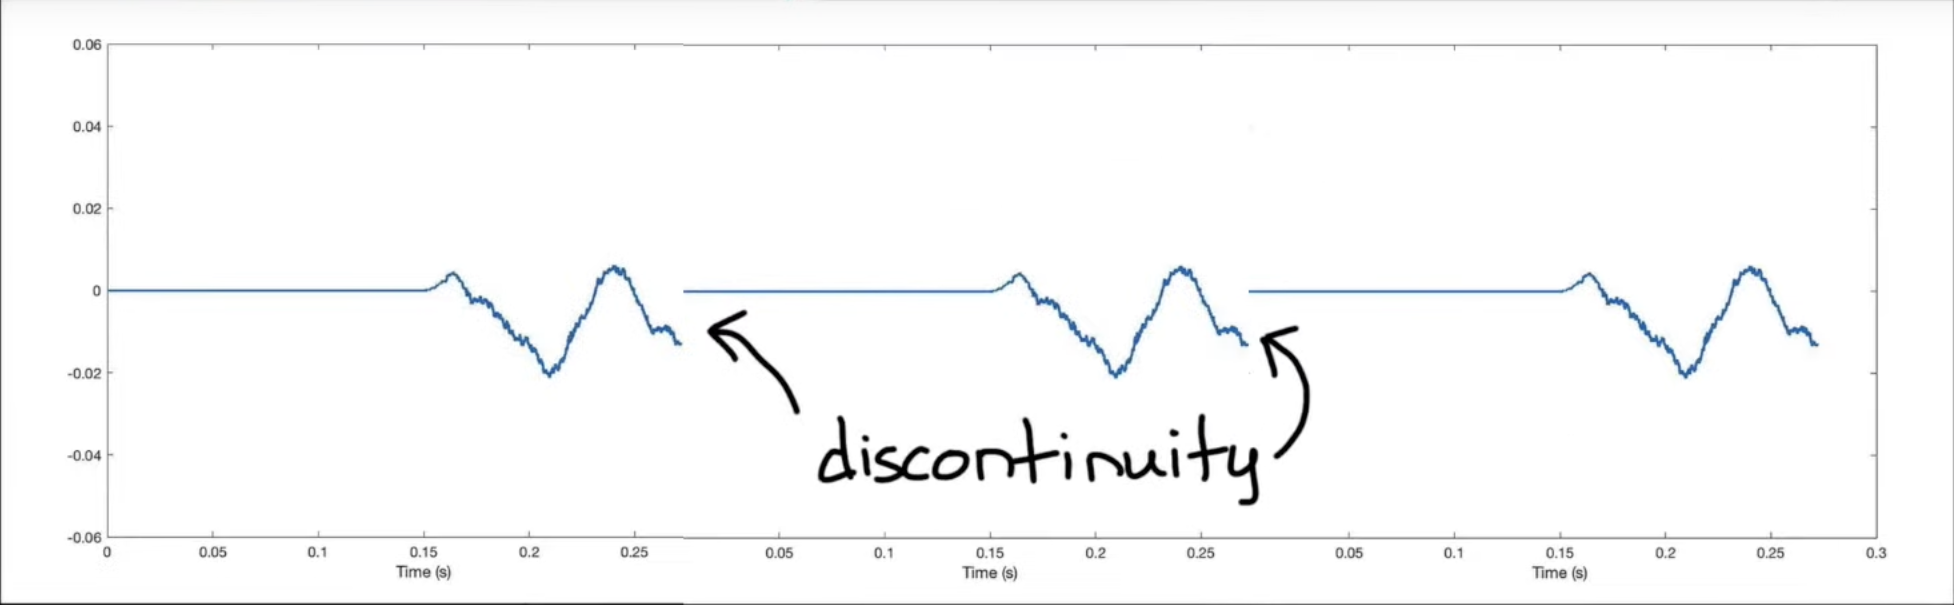
\includegraphics[width=0.5\linewidth]{discontinuity example.png}
    \label{fig:discon}
\end{figure}

After applying the STFT we now have frequency distribution for each segment of the data; however, this is still an excess of information needed for our model, we further decrease this by splitting the frequencies into a number of bins and taking a weighted average of each bin frequency amplitudes using a Mel Filter Bank. This reduces the STFT of each window to a much lower number of features, if 10 bins are used then we will have 10 values for each window. We then arrange these values in a 2 dimensional array to get a spectogram, where the x-axis represents the window number, and the y-axis shows the bin number for said window, and the value is the weighted average. This processed data can then be fed into our machine learning models. \\

\begin{figure}[h]
    \centering
    \caption{Example Spectrogram}
    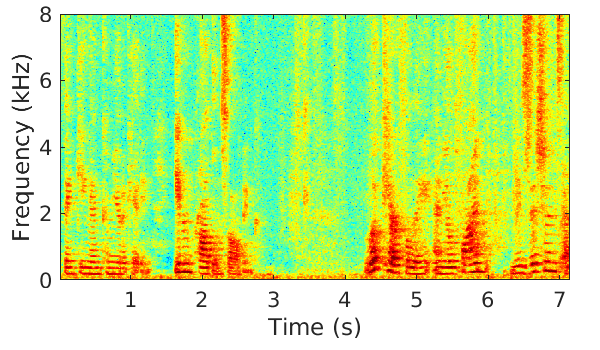
\includegraphics[width=0.5\linewidth]{example_spectrogram.png}
\end{figure}

\subsection{Filters}%
\label{subsec:filters}

Although going by with relatively little comment during the development process, it should be noted that currently all filters are invariant under permutations to time. Thus, while we can consider experiments such as taking higher order statistics of the sensor windows, a key concern is that no model can currently distinguish between processes moving forward in time vs. moving backwards, or indeed account whatsoever for the relative points in time at which events occur. This is particularly relevant for audio data, but also has an impact when we want gestures to represent particular types of changes as opposed states that are constantly occurring within each recording window. \\

Candidate solutions to this could involve introducing specific convolutional filters which may be activated or deactivated (e.g. have a convolution with a linearly increasing / decreasing function). This would also help to introduce a basic explanation of convolutional networks, while still remaining firmly within the domain that the application allows for.

\section{Concluding Remarks}%
\label{sec:conclusion}

Overall, this project has been largely successful in its goals. The given specification in section~\ref{subsec:spec} entailed that at least one additional sensor should be added. We added two, both of which are available for the user to choose before training, are visualised fully in the application, and cohere well with the existing ML models. Further, a third sensor (audio) was considered extensively, and we provide additional thoughts on how this could be implemented with more work in the future. The specification also stated that a new neural network architecture should be added, and of this we implemented the Mixture of Experts model, being both pedagogically useful by having clear corresponding real world analogies to its methodology, and performing reasonably well in the data context, even with relatively few examples. \\

We hope that our work is useful to the developers both at the Micro:Bit foundation, and at the CCTD of Aarhus University. Thanks in particular to Robert for his helpful guidance and organisation throughout this project, and to Qian for his work as our internal supervisor.

\bibliographystyle{IEEETran}
\raggedright\bibliography{main}

\end{document}
